\section{Classics}
\label{s:classics}
Various works that do not entirely rely on learning algorithms, be them deep or statistical, are reviewed.
The majority of these come from the pre deep learning era.
The discussion of this section is not strictly about the papers, but about the methodology of the time.

%%%%%%%%%%%%%%%%%%%%%%%%%%%%%%%%%%%%%%%%%
%              Hoeim
%%%%%%%%%%%%%%%%%%%%%%%%%%%%%%%%%%%%%%%%%
\subsection{Hoeim et al.}
Derek Hoeim and his collaborators produced a sequence of works on "scene interpretation" \cite{autopopup1, autopopup2, autopopup3, autopopup4, autopopup5, autopopup6}.
Only the first will be discussed in detail.

% example
\begin{figure}
	\centering
	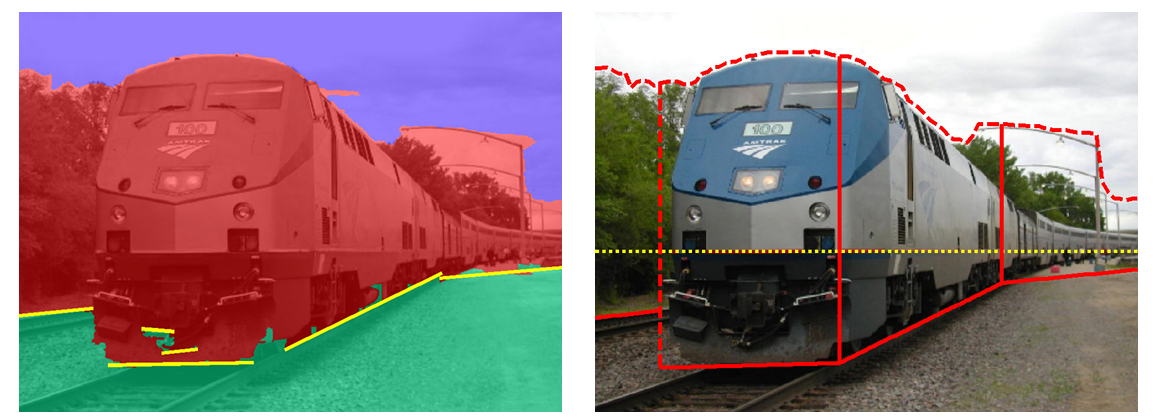
\includegraphics[scale=0.3]{figs/hoeim}
	\caption{Hoeim et al. method \cite{autopopup1}. Left: segmentation and lines fitting; Right: building the 3D model. \label{fig:hoeim}}
\end{figure}

In \cite{autopopup1} the objective is to do a simple reconstruction of the scene geometry by building a 3D model.
The reconstruction procedure is based on strong assumptions that are: the scene is composed by a ground, vertical objects stick to it and an infinite distant sky.
This obviously only work for outdoor scenes.
The ground is modeled as a plane and vertical objects as little segments of planes perpendicular to the ground and parallel to the image plane.
The pipeline is based on three phases:
\begin{enumerate}
	\item{Segmenting the image into "ground", "vertical" and "sky"}
	\item{Cleaning the segmentation}
	\item{Fitting lines to the segmented vertical regions and building the 3D model}
\end{enumerate}
In figure \ref{fig:hoeim} there is an example.
Another major assumptions is the absence of occlusion between objects.
If occlusion occurs, the segmentation procedure is not able to distinguish between different object by other means that some ground pixels in between.
Hence, in the case of occlusion, two objects at completely different depths would result in the closest to the camera.

Hoeim et al. deal with occlusion in \cite{autopopup4}, where they try to model the occlusion cues and build a computational method for occlusion detection.
The method uses a Conditional Random Field (CRF).
It was a very used statistical method in computer vision before deep learning, its main drawback is the expensive inference that involves a global optimization step.
In last years neural CRFs have been proposed also for single image depth estimation, although I will not review them.

In \cite{autopopup2} and \cite{autopopup5} the problem of the surface orientation prediction is tackled.
The idea, also found in older works like \cite{VideoCompass}, was to group surface normals into a predefined way.
For instance: pointing upward, pointing downward, pointing left or pointing right.
The result was a segmentation method.
At this time, for segmenting images, the main approach was to first do an over segmentation by dividing the image into super-pixels.
A super-pixels are groups of pixels that share some local property.
Second, associate to each super-pixel various numerical features, such as the histogram of colors, the number of pixels, the mean magnitude of the gradient, ...
These features were hand-crafted, in the sense that they are not learned and someone explicitly thought about them and tested them in some scenarios.
Doing so, each super-pixel has numbers associated to it.
Using a dataset of segmented images one could train a statistical learning method (e.g. a boosting method or a simple linear regression) to predict the correct labels for a given superpixel.
If the super-pixel information was not sufficient due to its locality, global optimization methods like Random Fields could have been used or iterative grouping (e.g. producing constellations of super-pixels by grouping them) was performed.

Continuing the journey of Hoeim et al., in \cite{autopopup3} the focus is on the objects.
In here object detection is tackled and the authors also attempt to orient detected objects in space.

All of these works lead to "Closing the Loop in Scene Interpretation" \cite{autopopup6} were they are all put together in a complex pipeline for building a 3D model of the scene as rich as possible.

%%%%%%%%%%%%%%%%%%%%%%%%%%%%%%%%%%%%%%%%%
%              Saxena
%%%%%%%%%%%%%%%%%%%%%%%%%%%%%%%%%%%%%%%%%
\subsection{Saxena et al.}
Saxena et al. go along the same journey and produce a series of papers \cite{saxena1, saxena2, saxena3, saxena4} which culminates in their master piece "Make3D: Learning 3D Scene Structure from a Single Still Image" \cite{saxena5}.
Their approach is based on Markov Random Field (MRF) models, that is a probabilistic model of the random fields family, as CRFs are.
Their idea is to over-segment the input image into super-pixels and consider them as small planar surfaces.
Planes on which super-pixels lay are modeled as 3-vectors and are the variables the MRF model has to optimize.
For defining a MRF, one has to define potential functions which define some quantity to be minimized.
In MRFs these potential functions depend on the super-pixel and its neighbours.
Saxena et al. encode the following property in the MRF model \cite{saxena5}:
\begin{itemize}
	\item{\textbf{Image features and depth:} the content of the super-pixel is correlated to its depth;}
	\item{\textbf{Connected structure:} except in the case of occlusion, neighboring super-pixels are more likely to be connected to each other;}
	\item{\textbf{Co-planar structure:} Neighboring superpixels are more likely to belong to the same plane if they have similar features and if there are no edges between them;}
	\item{\textbf{Collinearity:} Long straight lines in the image plane are more likely to be straight lines in the 3D model.}
\end{itemize}

For training the authors gather images inside the Standford campus and create the Make3D \cite{saxena5} dataset.
It is a small dataset compared to what's available today, but at the time it was an important benchmark.

Completing their work there is a 3D model construction based on the plane parameters inferred by the MRF model.
The 3D reconstruction is based on a mesh model of the super-pixels, which can also be textured using superpixel information and as shown in figure \ref{fig:saxena}.

% example
\begin{figure}
	\centering
	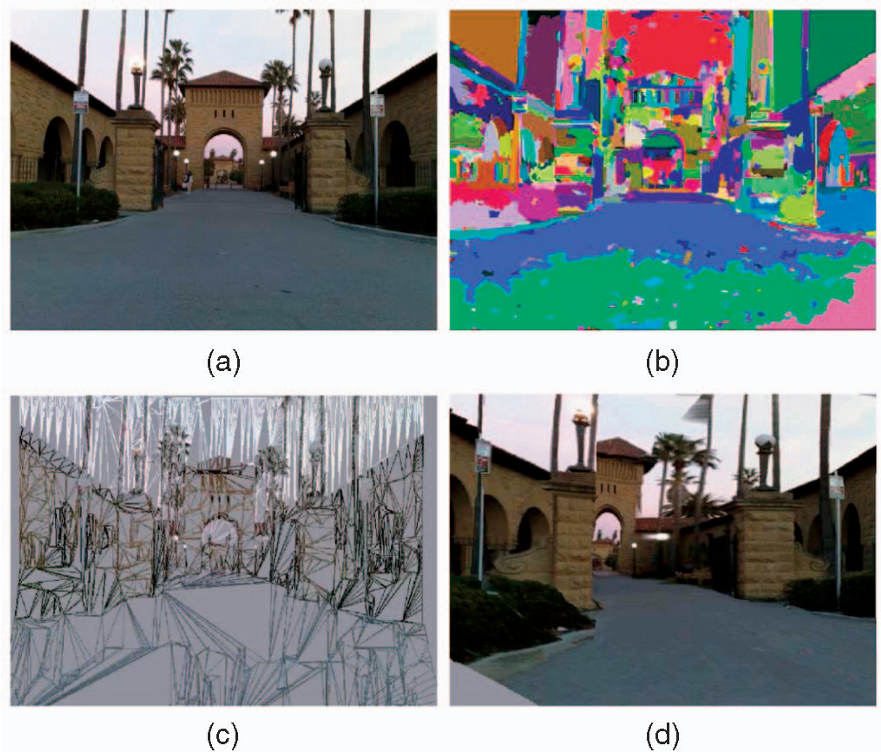
\includegraphics[scale=0.4]{figs/saxena}
	\caption{Saxena et al. example \cite{saxena5}. (a) The original image. (b) Over-segmentation of the image to obtain super-pixels. (c) The 3D model predicted by the algorithm. (d) A textured render of the 3D model. \label{fig:saxena}}
\end{figure}

%%%%%%%%%%%%%%%%%%%%%%%%%%%%%%%%%%%%%%%%%
%              DepthTransfer
%%%%%%%%%%%%%%%%%%%%%%%%%%%%%%%%%%%%%%%%%
\subsection{DepthTransfer}
Karsch et al. \cite{DepthTransfer} developed DepthTransfer for tackling the monocular depth estimation problem.
Their method can be thought of as a k-NN method.
The idea is to find k-nearest neighbors in the dataset, adapt them to the current image by warping and finally stitch together parts of each of them.
The nearest neighbor search is performed by extracting a lower dimensional representation of the image and defining some distance measure in that space.
So, for instance, if in the input image appears a car, it is very likely that an image with a car is part of its k-neighbors.
By warping the retrieved image, the two cars should approximately overlap and depth values can be "transferred" to the input image (hence the name of the method).
This idea was not invented by them and can also be found in works of Konrad et al. \cite{konrad1, konrad2}.
Karsch et al. main contribution is the depth fusion process of the neighbors.
In fact, previously given various depth maps to fuse the approach was to apply some averaging function pixel-wise, for instance in \cite{konrad2} the median of the depth values is taken and a post-processing filtering is applied thereafter.
An illustration of Karsch et al. method is in figure \ref{fig:depthtransfer}

% method
\begin{figure}
	\centering
	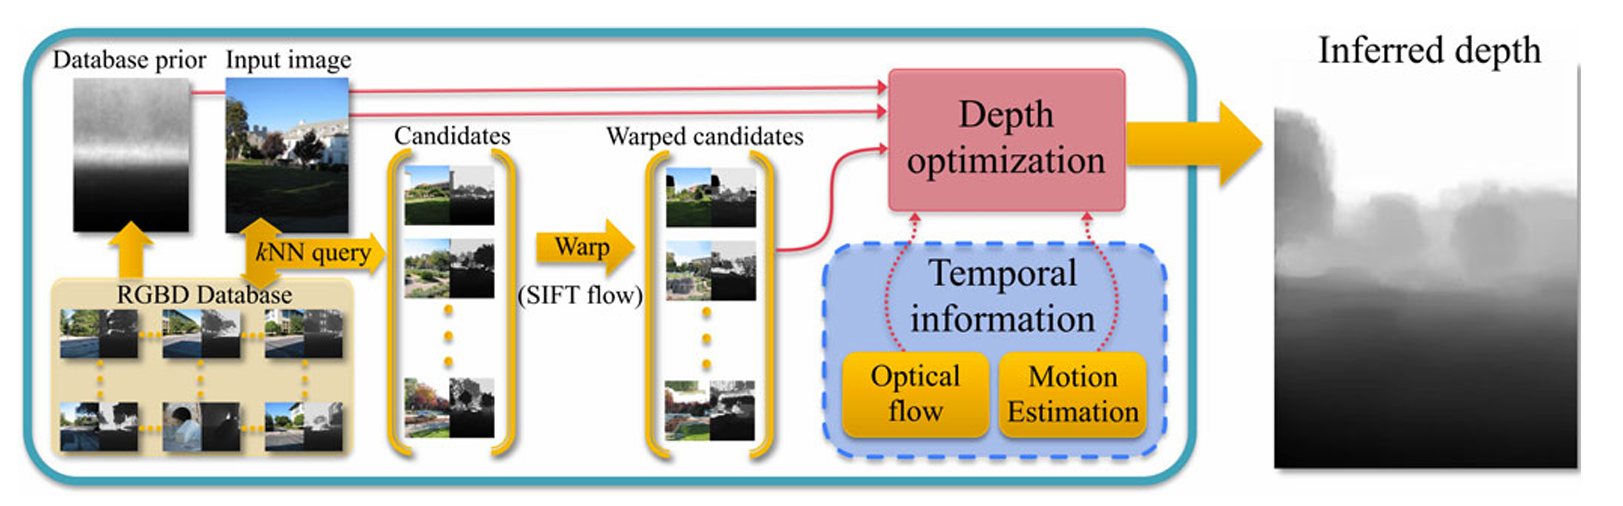
\includegraphics[scale=0.3]{figs/depthtransfer}
	\caption{Karsch et al. pipeline \cite{DepthTransfer}. The temporal information module that here appears serves the purpose to estimate depth of videos consistently predicting depth along the temporal dimension. Details are found in the paper \cite{DepthTransfer}. \label{fig:depthtransfer}}
\end{figure}

Before fusing the depth maps a preliminary warping is applied.
The warping is computed through SIFT Flow procedure \cite{SIFTFlow} that computes SIFT features pixel-wise and create a bijection between the pixels of the two images based on the computed features.
It is an expensive procedure though and today it could be substituted by some Optical Flow neural model.
After the warping is performed, the fusion is performed through a global optimization procedure which (simplifying) pixel-wise chooses from which image to take the depth value from.

%%%%%%%%%%%%%%%%%%%%%%%%%%%%%%%%%%%%%%%%%
%              IM2CAD
%%%%%%%%%%%%%%%%%%%%%%%%%%%%%%%%%%%%%%%%%
\subsection{IM2CAD}
This is the work on which I want to close this chapter.
It is from Izadinia et al. \cite{IM2CAD} and it is the direct evolution of the work from Lawrence Robert, whose quote starts the chapter.
Unlike the other papers discussed in this section, this uses deep learning and it is relatively recent (2017).
Nevertheless, its ideas are rooted in the visionary work of Lawrence Robert P.h.D. thesis, dated 1963.
Let's start immediately by looking at a representation of their inference pipeline in figure \ref{fig:im2cad}

% method
\begin{figure}
	\centering
	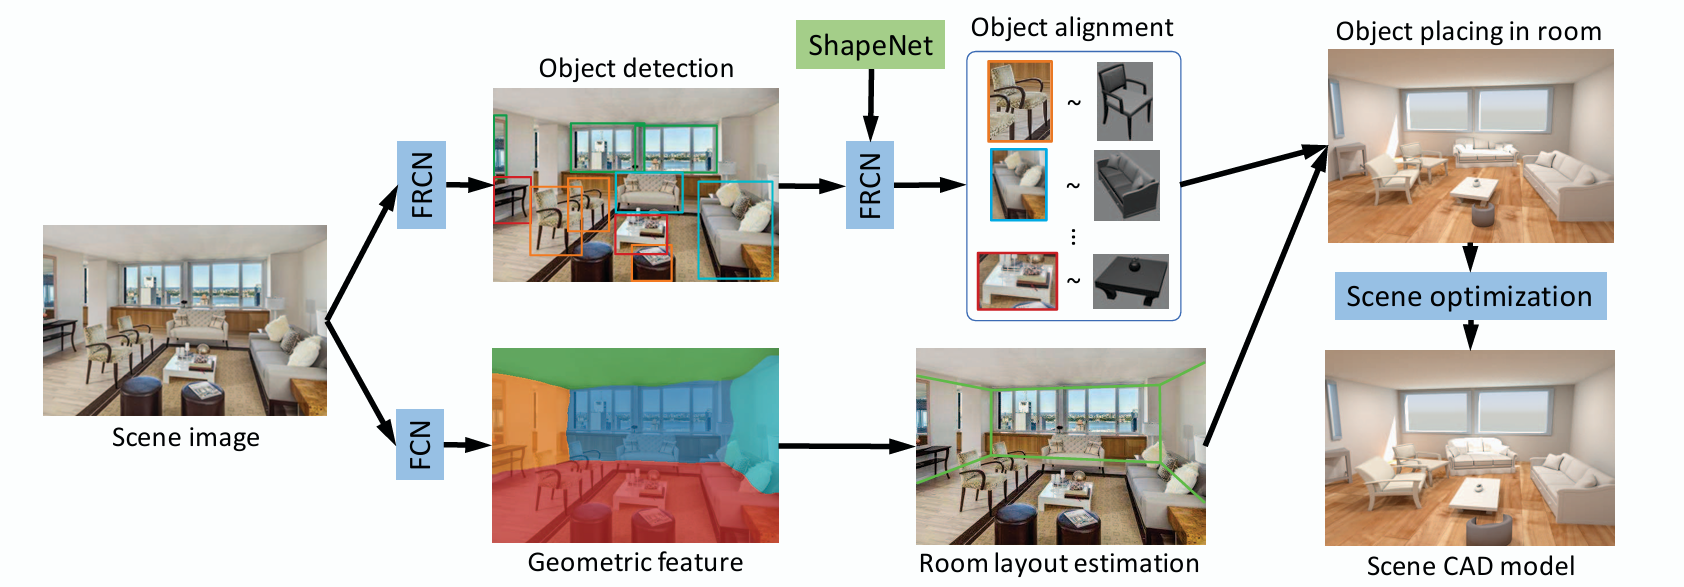
\includegraphics[scale=0.3]{figs/im2cad}
	\caption{Izadinia et al. \cite{IM2CAD} pipeline. \label{fig:im2cad}}
\end{figure}

First, it must be said that this method works exclusively in indoor environment that resemble the appearance of a "house room".
Similarly to what Hoeim et al. did in their method, here objects and background are treated separately.
There is a neural object detector that deals with furniture filling up the room and a neural segmentation model that subdivide the pixels into 5 categories corresponding to the 3 walls, the ceiling and the floor that a person can see by standing in a room.
This implies another limitation of the method: the room must have exactly 4 walls.
Now, a neural network compares the object detected with a CAD dataset of object appearances and match the detection with some real world 3D model of furniture by aligning its orientation in space.
Contemporary room layout estimation method builds a simple 3D model of the room.
Objects and room are now known.
The final step is to optimize the information found.
In order to do so, 3D models are placed in the room based on the initial guess given by the alignment procedure.
The 3D model is textured and rendered (illumination is given by windows and lights found in the room).
An iterative process compares the rendered view with the input image and adjusts the orientation, size and location of the objects until a criterion is fulfilled.
Eventually the scene CAD model is returned.